\documentclass[12pt,a4paper]{article}
\usepackage[utf8]{inputenc} %polskie znaki
\usepackage[T1]{fontenc}	%polskie znaki
\usepackage{amsmath}		%matematyczne znaczki :3
\usepackage{enumerate}		%Dodatkowe opcje do funkcji enumerate
\usepackage{geometry} 		%Ustawianie marginesow
\usepackage{graphicx}		%Grafika
\usepackage{wrapfig}		%Grafika obok textu
\usepackage{float}			%Allows H in figure
\usepackage{hyperref}		%Allows hyperlinks
%\pagestyle{empty} 			%usuwa nr strony
\usepackage{todonotes}		%Todo notatki
\usepackage{lipsum}         %Lorem text
\usepackage{ntheorem}   	% for theorem-like environments
\usepackage{mdframed}   	% for framing
\usepackage{subcaption}		% subfigure (image placing)
\usepackage{pdfcomment}		% Komentarze (z bazowego pdf'a)
\usepackage{xparse}			% New commands with optional arguments
\usepackage{ifthen}			% If then - funkcje!
\usepackage{expl3}			% Deklarowanie zmiennych
\usepackage{pgf}			% Aktualne rachunki \pgfmathparse{}
\usepackage{amsmath} 		% For mathematical symbols and structures
\usepackage{amsfonts}		% Zbiór liczb naturalnych + formatowanie
\usepackage{ulem}			% Przekreślony text
%\usepackage[colorlinks=true, linkcolor=blue, urlcolor=red, citecolor=green]{hyperref}
\usepackage{fontawesome5}
\usepackage{mathtools}

\newgeometry{tmargin=2cm, bmargin=2cm, lmargin=2cm, rmargin=2cm} 

%Counter commands{
	\newcounter{definicja}
	\setcounter{definicja}{1} 
	\newcounter{twierdzenie}
	\setcounter{twierdzenie}{1} 
	\newcounter{przyklady}
	\setcounter{przyklady}{1} 
	\newcounter{wnioski}
	\setcounter{wnioski}{1} 
	
	\newcommand{\counter}[1]{
		\arabic{#1} \stepcounter{#1} 
	}
	\newcommand{\counterreset}[1]{\setcounter{#1}{1}}
	%}

%Define styles{
	\theoremstyle{break}
	\theoreminframepreskip{0.5cm}
	\theoremheaderfont{\bfseries}
	\newmdtheoremenv[%
	linecolor=white,%
	innertopmargin=\topskip,
	shadowsize=0,%
	innertopmargin=5,%
	innerbottommargin=5,%
	leftmargin=10,%
	rightmargin=10,%
	backgroundcolor=gray!20,%
	innertopmargin=0pt,%
	ntheorem]{zad}{Zadanie}
	
	\mdfdefinestyle{zadanie}{
		linecolor=white,%
		innertopmargin=5,%
		innerbottommargin=5,%
		leftmargin=10,%
		rightmargin=10,%
		backgroundcolor=gray!20,%
		innertopmargin=8,
		innerbottommargin=8,
		skipabove = 5,
	}
	\mdfdefinestyle{wzor}{
		linecolor=cyan,%
		linewidth=2pt,%
		innertopmargin=8,
		innerbottommargin=8,
		leftmargin=10,%
		rightmargin=10,%
		backgroundcolor = white, 
		fontcolor = black,
		skipabove = 5,
		skipbelow = 5,
	}
	%}

%Zadania templatex%{
	\newcommand{\Obramowka}[1]{
		\begin{mdframed}[style=wzor]
			\centering #1
		\end{mdframed}
	}
	\newcommand{\Komentarz}[1]{
	\begin{mdframed}[style=zadanie]
		\textbf{Komentarz}\\
		#1
	\end{mdframed}
	}
	
	%}

% Set spacing before and after theorems
\setlength{\theorempreskipamount}{20pt}  % Space above the theorem
\setlength{\theorempostskipamount}{20pt} % Space below the theorem

\newtheorem{definition}{Definicja}[section]

\newtheorem{theorem}{Twierdzenie}[section]
\newtheorem{lemma}{Lemat}[section]
\newtheorem{wniosek}{Wniosek}[theorem]
\newtheorem{example}{Przykład}[section]
\newtheorem{exercise}{Ćwiczenie}[section]
\newtheorem{stwierdzenie}{Stwierdzenie}[section]
\newtheorem{obserwacja}{Obserwacja}[section]


%\newcommand{\endproof}{\begin{flushright}\square\end{flushright}}
\newcommand{\tg}{\text{tg}}
\newcommand{\ctg}{\text{ctg}}
\newcommand{\witw}{$\Leftrightarrow$}
\newcommand{\wynika}{$\Rightarrow$}
\newcommand{\UkladRownan}[2]{
	$\left\{
	\begin{array}{l}
		#1 \\
		#2
	\end{array}
	\right.$
}

\begin{document}
	% Strona tytułowa
	
	% Dodanie strony tytułowej
	\begin{titlepage}
		\centering
		\vspace{1cm}
		{\Huge\bfseries Matematyczne aspekty wyborów \par} 
		\vspace{1.5cm}
		{\large Na podstawie wykładu \par} 
		\vspace{0.5cm}
		{\Large Krzysztofa Ciesielskiego}\\
		\vspace{1cm}
		{\large Skrypt autorstwa}\\
		\vspace{0.5cm}
		{\Large Arkadiusza Dąbala}\\
		\vfill 
		{\large Wersja z dnia:}\\
		{\Large \today \par}  
		\vspace*{1cm}
	\end{titlepage}
	\newpage
	\tableofcontents
	\newpage
\section{Preliminaria}
\subsection{Jak wyglądają aktualnie wybory?}
\Komentarz{Materiał ten nie ma w żadnym stopniu charakteru politycznego, a wyłącznie charakter matematyczny.}

\begin{example}
Rozważmy poniższe dane, oparte na 6 partiach, 1000 głosach i 6 mandatów do rozdania:
\end{example}

\begin{tabular}{|c|c|c|c|c|c|c|}\hline
	Nazwa        & Głosy & $:1$ & $:2$ & $:3$ & $:4$ & Otrzymane mandaty\\\hline
	Filateliści  & 380   & \textbf{380} & \textbf{190} & \textbf{127} & 87   & 3\\\hline
	Gitarzyści   & 192   & \textbf{192} & \textbf{96}  & 64   &       & 2\\\hline
	Szachiści    & 180   & \textbf{180} & 90    &       &       & 1\\\hline
	Piłkarze     & 96    & \textbf{96}  & 48    &       &       & 1\\\hline
	Lotniarze    & 90    & 90    &       &       &       & 0\\\hline
	Kolejarze    & 62    & 62    &       &       &       & 0\\\hline
\end{tabular}\\

System ten działa w następujący sposób:

\begin{itemize}
	\item Liczby głosów dzielone są przez kolejne liczby naturalne dodatnie (tak jak w tabeli).
	\item Wybierane są z tej tabeli 6 największych liczb (wytłuszczony druk).
	\item Liczba mandatów zależy od liczby wytłuszczonych liczb w wierszu partii.
\end{itemize}

\begin{example}
	Rozważmy tę samą tabelę, ale załóżmy, że partia \textbf{Gitarzyści} nie przekroczyła progu $5\%$.
\end{example}

\begin{tabular}{|c|c|c|c|c|c|c|}\hline
	Nazwa        & Głosy & $:1$ & $:2$ & $:3$ & $:4$ & Otrzymane mandaty\\\hline
	Filateliści  & 380   & \textbf{380} & \textbf{190} & \textbf{127} & 87   & 3\\\hline
	\sout{Gitarzyści}  & \sout{192}  & \sout{192} & \sout{96}  & \sout{64}  & \sout{---} & \sout{---} \\\hline
	Szachiści    & 180   & \textbf{180} & \textbf{90}  &       &       & 2\\\hline
	Piłkarze     & 96    & \textbf{96}  & 48    &       &       & 1\\\hline
	Lotniarze    & 90    & \textbf{90}  &       &       &       & 1\\\hline
	Kolejarze    & 62    & 62    &       &       &       & 0\\\hline
\end{tabular}\\

\begin{example}
	Rozważmy następującą tabelę z 5 mandatami do rozdania:
\end{example}

\begin{tabular}{|c|c|c|c|c|c|}\hline
	Nazwa    & Głosy $:1$ & $:2$ & $:3$ & $:4$ & Mandaty\\\hline
	Rybacy   & \textbf{6000} & \textbf{3000} & \textbf{2000} & 1500 & 3\\\hline
	Myśliwi  & \textbf{5700} & \textbf{2850} & 1900  &       & 2\\\hline
	Artyści  & 1950          & 975           &       &       & 0\\\hline
\end{tabular}\\

Partia \textbf{Rybacy} prowadziła kampanię przeciwko \textbf{Myśliwym}, w wyniku czego liczba otrzymanych głosów zmieniła się następująco:
\begin{itemize}
	\item Partia \textbf{Rybacy} zyskała 400 głosów (+400)
	\item Partia \textbf{Myśliwi} straciła 600 głosów (-600)
	\item Partia \textbf{Artyści} zyskała 200 głosów (+200)
\end{itemize}

\begin{tabular}{|c|c|c|c|c|c|}\hline
	Nazwa    & Głosy $:1$ & $:2$ & $:3$ & $:4$ & Mandaty\\\hline
	Rybacy   & \textbf{6400} & \textbf{3200} & 2133 &       & 3\\\hline
	Myśliwi  & \textbf{5100} & \textbf{2550} & 1700 &       & 2\\\hline
	Artyści  & \textbf{2150} & 1075          &      &       & 0\\\hline
\end{tabular}\\

\Komentarz{Tym oto sposobem partia \textbf{Myśliwi} stracili jeden mandat na rzecz partii \textbf{Artyści}.}

\begin{example}
	Rozważmy wyniki głosowania dla dwóch partii z 6 mandatami do rozdania.
\end{example}

\begin{tabular}{|c|c|c|c|c|c|c|}\hline
	Nazwa        & Głosy $:1$ & $:2$ & $:3$ & $:4$ & $:5$ & Mandaty\\\hline
	Matematycy   & \textbf{1200} & \textbf{600} & \textbf{400} & \textbf{300} & \textbf{240} & 5\\\hline
	Politycy     & \textbf{201}  & 101         &       &       &       & 1\\\hline
\end{tabular}\\

Popatrzmy na głosy bezpośrednio na konkretnych kandydatów z każdej partii:

\begin{tabular}{|c|c|}\hline
	Nazwa   & Głosy\\\hline
	Kwadrat & \textbf{201}\\\hline
	Trójkąt & \textbf{200}\\\hline
	Stożek  & \textbf{200}\\\hline
	Walec   & \textbf{200}\\\hline
	Suma    & \textbf{200}\\\hline
	Iloczyn & 199\\\hline
\end{tabular} $\qquad\qquad\qquad\qquad\qquad$
\begin{tabular}{|c|c|}\hline
	Nazwa        & Głosy\\\hline
	Magister     & \textbf{35}\\\hline
	Magistra     & 34\\\hline
	Urzędnik     & 33\\\hline
	Urzędas      & 33\\\hline
	Pani Basia   & 33\\\hline
	Pan Andrzej  & 33\\\hline
\end{tabular}\\

\Komentarz{Tym oto sposobem mandatu nie otrzymuje \textbf{Iloczyn}, mimo że zdobył więcej głosów niż \textbf{Magister}.}

\begin{example}
	Rozważmy sytuację, w której państwo jest podzielone na dwa bloki, oba mające po $50\%$ wpływu na wyniki wyborów. Każdy blok ma przyznać po 4 mandaty.
\end{example}

\begin{center}
	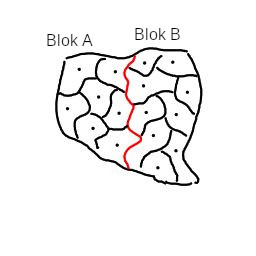
\includegraphics{5050.jpg}
\end{center}

W bloku A znajdowały się dwie partie: PZK (Partia Zwolenników Kawy) i PZH (Partia Zwolenników Herbaty), z których każda otrzymała po 25\% głosów w ogólnokrajowym głosowaniu. W bloku B znajdowała się partia PZA (Partia Zwolenników Alkoholu) oraz inne partie, które nie przekroczyły progu 5\%. Przedstawmy liczbę uzyskanych głosów w PZA:

\begin{tabular}{|c|c|}\hline
	Nazwa       & Głosy\\\hline
	Żubr        & \textbf{19995}\\\hline
	Żubrówka    & \textbf{2}\\\hline
	Soplica     & \textbf{2}\\\hline
	Pan Tadeusz & \textbf{1}\\\hline
\end{tabular}\\

\Komentarz{I tym oto sposobem wygrywają osoby, które dostają 2 lub 1 głos.}

\subsection{\href{http://www.racjonalista.pl/kk.php/s,9848/k,3}{Prawo Ciesielskiego}}

Rozważmy głosowanie względem 2 partii z 7 mandatami:

\begin{tabular}{|c|c|c|c|c|c|c|}\hline
	Nazwa        & Głosy:1 & :3 & :5  & :7  & :9  & Mandaty\\\hline
	Kelnerzy     & \textbf{1050} & \textbf{350} & \textbf{210} & 150 & 117  & 4\\\hline
	Sportowcy    & \textbf{1008} & \textbf{336} & 202  & 144 &      & 3\\\hline
\end{tabular}\\

Partia \textbf{Sportowcy} postanowiła się rozdzielić na dwie partie i startować osobno:

\begin{tabular}{|c|c|c|c|c|c|c|}\hline
	Nazwa        & Głosy:1 & :3 & :5  & :7  & :9  & Mandaty\\\hline
	Kelnerzy     & \textbf{1050} & \textbf{350} & \textbf{210} & 150 & 117  & 3\\\hline
	Piłkarze     & \textbf{504}  & \textbf{168} & 101  &     &      & 2\\\hline
	Siatkarze    & \textbf{504}  & \textbf{168} & 101  &     &      & 2\\\hline
\end{tabular}\\

\Komentarz{Tym oto sposobem partia \textbf{Sportowcy} zdobyła większość.}

	
\newpage

\section{Treść właściwa}
\subsection{Metody głosowania (system wyborczy)}

Wprowadźmy kilka oznaczeń, niech: \\
\\ $W$ - zbiór wszystkich wyborców, \\
$K$ - zbiór wszystkich kandydatów.
\begin{itemize}
	\item Ten sam układ głosów (zestaw głosów) daje ten sam wynik (funkcja).
	\item Każdy układ głosów daje jakiś wynik (może być $\emptyset$).
\end{itemize}

\begin{definition}[Model]
	Model to układ głosów (z przyporządkowanymi wyborcami).
\end{definition}

\begin{definition}[Metoda anonimowa]
	Metoda jest anonimowa, \textit{wtedy i tylko wtedy} (w skrócie: \witw), gdy wszyscy wyborcy są traktowani tak samo, \witw $\forall_{x,y \in W}$ zamiana głosów $x$ i $y$ nie zmienia wyniku.
\end{definition}

\Komentarz{Alternatywnie, metoda nie jest anonimowa \witw $\exists_{x,y \in W}$ takie, że zamiana głosów $x$ i $y$ \textit{istotnie} zmienia wynik.}

\begin{definition}[Metoda neutralna]
	Metoda jest neutralna, \witw wszyscy kandydaci są traktowani tak samo, \witw $\forall_{x,y \in K}$ zamiana ról $x$ i $y$ nie zmienia wyniku.
\end{definition}

\Komentarz{Alternatywnie, metoda nie jest neutralna \witw $\exists_{x,y \in K}$ takie, że zamiana ról $x$ i $y$ \textit{istotnie} zmienia wynik, dokładniej definiując:\\
jeśli $\exists{k_1,k_2\in K}: W_1=\{w_{1},w_{2},\dots,w_{i}\}$ głosowali na $k_1$, a $W_2=\{w_{i+1},w_{i+2},\dots,w_{j}\}$ głosowali na $k_2$ to jeżeli kandydaci Ci "zamienią się" wyborcami (zbiorami $W_1,W_2$), to $k_1$ i $k_2$ zamienią się wynikami.}

\begin{definition}
	Trzy rodzaje metod ze względu na wyniki:
\end{definition}

\begin{enumerate}[1)]
	\item Metoda zwycięzcy (MZ) – wybiera zwycięzcę (zwycięzców),
	\item Metoda porządkowa (MP) – wynik to słaby porządek na zbiorze $K$,
	\item Metoda rozdziału (MR) – wynik to podział pewnych dóbr między kandydatów.
\end{enumerate}
\subsubsection{Metoda zwyciężcy}
\begin{definition}[Klasyczna metoda zwycięzcy]
	Klasyczna metoda zwycięzcy (klasyczna MZ) polega na tym, że każdy wyborca głosuje na dokładnie jednego kandydata. Zbiór
	$$\Sigma = \{m:W\rightarrow K\}$$
	jest zbiorem modeli, gdzie $m$ jest modelem. Klasyczną metodę zwycięzcy możemy opisać funkcją
	$$f: \Sigma \rightarrow P(K).$$
\end{definition}

\begin{definition}[Semi-klasyczna metoda zwycięzcy]
	Semi-klasyczna MZ polega na tym, że każdy wyborca głosuje na co najmniej jednego kandydata:
	$$\Sigma = \{m:W\rightarrow P(K)\setminus \emptyset\}.$$
	Metodę tę można opisać funkcją
	$$f: \Sigma \rightarrow P(K).$$
\end{definition}

\begin{definition}[Metoda efektywna]
	Metoda zwycięzcy jest efektywna \witw zawsze wyłania przynajmniej jednego zwycięzcę.
\end{definition}

\begin{example}[Przykłady metod głosowania]
	\textbf{Metody klasyczne:}
\end{example}
\begin{enumerate}[1)]
	\item Dyktatura – $\exists_{\;p \in W}$: wynik jest tożsamy z głosem $p$.
	\item Monarchia – dany kandydat $k \in K$ wygrywa niezależnie od głosowania.
	\item Metoda większości – wygrywa kandydat (lub kandydaci), który(a) otrzymał(a) najwięcej głosów.
	\item Metoda bezwzględnej większości – wygrywa kandydat $k \in K$, który otrzymał co najmniej $\lfloor\frac{\# W}{2}\rfloor + 1$ głosów.
	\item Metoda super większości – wygrywa kandydat, który uzyskał co najmniej $q$ głosów, gdzie $q > \frac{\# W}{2}$.
	\item Metoda status quo – \textit{Założenie:} $\exists$ pewien stan z jednym zwycięzcą.
	\\ Głosowanie metodą większości (lub super większości):
	\begin{itemize}
		\item jeśli metoda daje wynik, zwycięża "nowy" kandydat,
		\item jeśli metoda nie daje wyniku, zwycięża dotychczasowy kandydat.
	\end{itemize}
	Przykład: referendum.
	\item Metoda większości ważonej – $(W = \{a_1,\dots,a_n\})$, gdzie głos $a_i$ ma wagę $w_i \geq 0$. Wygrywa ten, kto otrzyma ponad $\frac{w_1 + \dots + w_n}{2}$ punktów.
	\item Metoda głosowania blokowego – $W = W_1 \cup \dots \cup W_n$, gdzie $W_k$ to zbiór wyborców bloku. $W_k$ podejmuje decyzję większością głosów. W przypadku remisu wybierają zwycięzcę w $W_k$. Głos z $W_k$ ma wagę $i_k$. Wygrywa kandydat z największą liczbą punktów.
	
	\textbf{Metody semi-klasyczne:}
	\item Metoda n-głosów – każdy wyborca głosuje na $n$ kandydatów, a zwycięża ten, kto uzyska najwięcej głosów.
	\item Szeroka metoda n-głosów - każdy głosuje na n kandydatów, ale mamy n zwyciężców (lub więcej w przypadku remisu na ostatnim "wygrywającym" miejscu)
	
	\textbf{Metoda ani klasyczna, ani semi-klasyczna:}
	\item Metoda punktowa – każdy wyborca $w \in W$ ma do rozdysponowania $p$ punktów $(p \in \mathbb{N})$ między kandydatów. Zwycięża kandydat z największą liczbą punktów.
\end{enumerate}

\begin{definition}[Metoda decyzyjna]
	Metoda zwycięzcy jest decyzyjna \witw w każdym modelu wyłania dokładnie jednego zwycięzcę.
\end{definition}

\begin{definition}[Metoda prawie decyzyjna]
	Metoda zwycięzcy jest prawie decyzyjna \witw w każdym modelu wyłania co najwyżej jednego zwycięzcę. Sytuacja, w której nie ma zwycięzcy, zachodzi wtedy, gdy więcej niż jeden kandydat uzyskał tę samą, najwyższą liczbę punktów.
\end{definition}

\begin{exercise}[Z ćwiczeń]
	Zbadaj kto jest zwycięzcą w głosowaniu przez 99 osób na kandydatów: \textbf{Anastazy}, \textbf{Bermudy}, \textbf{Cezary}, jeśli otrzymano następujące wyniki metodą porządkową:
\end{exercise}

	\begin{tabular}{|c|c|}\hline
		Liczba głosów	& Wynik porządkowy\\\hline
		18        		& ABC\\\hline
		15    			& ACB\\\hline
		24     			& BAC\\\hline
		8 				& BCA\\\hline
		16     			& CAB\\\hline
		18 				& CBA\\\hline
	\end{tabular}\\
	
\begin{exercise}
	Dane są wyniki głosowania:\\\\
	\begin{tabular}{|c|c|}\hline
		Imię		& Liczba głosów\\\hline
		Jaś        	& 100\\\hline
		Małgosia    & 1\\\hline
	\end{tabular}\\\\
	Zrób tak, by Małgosia wygrała.
\end{exercise}

\begin{exercise}
	Uzupełnij tabelę:\\
	\begin{tabular}{|c|c|c|c|}\hline
		& Anonimowa & Neutralna & Efektywna\\\hline
		Dyktatura   &&&\\\hline
		Monarchia   &&&\\\hline
		Metoda Większości &&&\\\hline
	\end{tabular}\\
\end{exercise}

	\begin{definition}[Kryterium jednoznacznej bezwzględnej większości]
		Metoda zwyciężcy (MZ) spełnia kryterium jednoznacznej bezwzględnej większości \witw kandydat który ma ponad 50\% głosów jest jedynym zwyciężcą. 
	\end{definition}
	
	\begin{stwierdzenie}
	Mamy klasyczną metodę zwyciężcy, taką że $\# K=2$ i głosowanie jest metodą bezwględnej większości, wówczas metoda jest prawie decyzyjna.
	\begin{enumerate}[1$^\circ$]
		\item $\# W$ nieparzysta - OK.
		\item $\# W$ parzysta:
		\begin{itemize}
			\item jeden ma więcej niż 50\% - OK.
			\item równa 50\% - nie ma zwyciężcy.
		\end{itemize}
	\end{enumerate} TODO(endproof)
	\end{stwierdzenie}
	
	
						
	\begin{stwierdzenie}
		Metoda jest decyzyjna $=>$ metoda jest prawie decyzyjna.
	\end{stwierdzenie}
	\newpage
	\begin{definition}[Metoda monotoniczna ze względu na zwyciężcę]
		\textbf{Z:} MZ - klasyczna lub semi-klasyczna.
		Metoda jest monotoniczna ze względu na zwyciężcę \witw Kandydat A wygrywa oraz $B\neq A$ grupa wyborców zamieni A i B rolami bez straty dla A
		Jeżeli model się zmieni przy następujących dozwolonych operacjach: 
		
		\begin{tabular}{|c|c|c|}\hline
			M & $\Rightarrow$ & N\\\hline
			A B & $\Rightarrow$ & A B\\\hline
			- - & $\Rightarrow$ & - -\\\hline
			+ + & $\Rightarrow$ & + +\\\hline
			- + & $\Rightarrow$ & + -\\\hline
		\end{tabular}
		
		\begin{itemize} 
			\item B -> A
			\item 0 -> 0
			\item 0 -> 1
			\item 1 -> 1 
		\end{itemize}
		
		$\Rightarrow$ A dalej wygrywa.
	\end{definition}
	
	\begin{definition}[Metoda quoty]
		MZ klasyczna lub semi-klasyczna jest metodą quoty (większości kwalifikowanej) \witw $\exists_q$ (quota) - liczba głosów o własności: kandydat A jest zwyciężcą \witw A dostał conajmniej $q$ głosów.\\
		
		(Często quota wyrażana jest w procentach, wtedy nieraz z nierównością słabą.)
	\end{definition}
		
		\begin{theorem}[Maya - \textit{Kenneth Maya, 1952r}]
			Z: Klasyczna metoda zwyciężcy i $\# K = 2$, metoda, która jest:
			\begin{itemize}
				\item anoniowa 
				\item neutralna
				\item monotoniczna ze względu na zwyciężce
				\item prawie decyzyjna
			\end{itemize}
			$\Rightarrow$ jest metodą bezwzględnej większości.
		\end{theorem}
		Złóżmy, że $A,B$ - kandydaci
		Metoda aninimowa $\Rightarrow$ interesuą nas liczby głosów
		A - a głosów
		B - b głosów
		1* $\# W = 2n$ (parzysta) a=n, b=n
		1.1Hipoteza A wygrywa metoda jest neutralna, to przy wymianie wyborców $\Rightarrow$ B wygyrwa $\Rightarrow$ A,B wygyrwają sprzeczność
		
		Analogicznie B nie wygyrwa 			(żadej nie ma ponad 50\%, nie ma wyższych)
		
		
		1.2* a>b, Hipoteza: B wygrywa, a-b wyborców zmiania głosy z B na A z monotoniczności $\Rightarrow$ B dalej wygrywa
		
		B ma teraz a głosów $\Rightarrow$(neutralność) A ten wygrywa -> sprzeczność z prawie decyzyjne
		
		prawie decyzyjne $\Rightarrow$ A wygyrwa
		
		A ma ponad połowę głosów
		
		2* $\# W = wn+1$ (nieparzyście)
		
		Niech a>b ipoteza B wygyrwa, a-b TODO zmienią głosy i jak poprzednio udowadniamy
		
		Zawsze wygyrwa ten co ma ponad połowę głosów.
		
		
	
		\begin{definition}[Metoda zakładająca uporządkowanie]
			Metoda zwyciężcy jest metodą zakładającą uporządkowanie (MZU) \witw $\forall_{w\in W}$ ustala K kandytatów w niliowym porządku i od tego zależy jego głos.
		\end{definition}
		Zapis $A\overset{w,m}{<}B$ w modelu $m$, wstawia $B$ wyżej niż $A$\\
		$A\overset{w}{<}B$ - gdy wiadomo jaki model
		
		
		
		\begin{example}
			\begin{enumerate}[1.]
				\item Metoda punktów Bordy (Jean Charles de Borda - 1733 - 1799 - Inżynier wojskowy)  - Każdy wyborca punktuje od (n-1) do 0 
				1. n-1
				2. n-2
				$\vdots$
				n-1 - 1
				n - 0
				wygrywa ten co otrzyma największą liczbę punktów
				\item Metoda Hare'a (Sir Thomas Hare 1806 - 1891 - Anglia, Prawnik) - (1857r) polega na odrzucaniu tego (tych), kto ma najmniej pierwszych miejsc i głosujemy dalej (listy pozostają z usunięciem odrzuconego kandydata) aż ktoś ma ponad $50\%$. Gdy równo i nie ma kogo odrzucić wtedy wszyscy wygrywają.
				\item Metoda Coombs'a (Clyde Coombs - 1912 - 1988, USA, Psycholog) - wypisujemy kolejność, odrzucamy tego, kto ma najwięcej ostatnich miejsc i głosujemy dalej aż ktoś ma ponad $50\%$ pierwszych miejsc.  Gdy się nie da wyrzucać, wygrywają wszyscy, którzy zostali.
				\item Metoda odrzuceń ostatniego - jak w metodzie Coombsa, przy czym odrzucamy "do oporu".  Gdy się nie da wyrzucać, wygrywają wszyscy, którzy zostali.
				
				\begin{example}
					Różnica między metodą Coomb'sa,a metodą odrzucania.
					TABELKA
				\end{example}
				
				\item Metoda Copelanda (Arthur H Copeland - 1898 - 1970 - Matematyk) - porównujemy parami kandydatów. Ten który więcej razy wyżej 1 pkt, w przypadku remisu po 0.5 punktu. 
				
				$\#{m:A\overset{m}{<}B}$\\
				$\#{m:B\overset{m}{<}A}$
				
				Decyduje suma punktów. (Zwyciężców może być więcej niż 1)
				
				\item Metoda terminażowa (Z: $\# W = 2n+1$ nieparzysta) - $k_1$ porównujemy z $k_2$ (metodą powyżej), następnie porównujemy z $k_3$ itd.
				
				\item Metoda pozycyjna - $P(p_1, p_2, \dots , p_n)$ przy czym $p_1\geq p_2 \geq \dots \geq p_n$. 
				1 - $p_1$ punktów
				2 - $p_2$ punktów itd.
				Wygrywa ten z największą ilością punktów. 
			\end{enumerate}
			\textbf{UWAGA - w szczególności:} 
			Metoda Bordy: $P(n-1, n-2,\dots, 1, 0)$
			Metoda większości $P(1,0, \dots , 0)$
			Metoda k głosów $P(1,1,\dots, 1, 0, \dots, 0)$ (gdzie 1 występuje k razy)
			
		\end{example}
	\newpage
	\section{Deser}
	W sumie to deseru jeszcze nie ma, ale ma być na ostatnim wykładzie!!! 
		
	\begin{center}
		 {\fontsize{30}{36}\selectfont\faBirthdayCake}
	\end{center}
	

	
	
\end{document}